\documentclass{report}
\usepackage[spanish]{babel}
\usepackage[utf8]{inputenc}
\usepackage{graphicx, longtable, float, titlesec, hyperref, xcolor}
\usepackage[margin=3cm]{geometry}

\hypersetup{
    hidelinks = true
}

\titleformat{\chapter}[display]
  {\normalfont\bfseries}{}{0pt}{\Huge}

\begin{document}
    \begin{titlepage}
        \centering
        
\includegraphics[width=0.6\textwidth]{./img/miscelanio/logo.jpg}\\
        \vspace{1cm}
        \LARGE Sistemas de Gestión de Seguridad de Sistemas de Información\\
        \vspace{0.5cm}
        \Large Ingeniería Informática de Gestión y Sistemas de Información\\
        \vspace{3cm}
        \Huge Sistema Web\\
        \vspace{2.5cm}
        \Large Autores:\\
        \vspace{0.2cm}
        \large Xabier Gabiña\\
        \large Ainhize Martinez\\
        \large Marcos Martín\\
        \vfill
        \today
    \end{titlepage}
    \tableofcontents
    \chapter{Introducción}
    \chapter{Vulnerabilidades}
        \section{Rotura de control de acceso}
            \subsection{Acceso mediante URL}
                Es posible publicar contenido en la pagina web mediante el uso de la URL.
                Para ello, basta con acceder a la pagina de creacion de eventos y mandar una peticion POST con los datos del evento.
                Para ello, podemos usar la herramienta curl de la siguiente forma:\\

                \begin{center}
                    \texttt{curl -X POST -d "titulo=Prueba\&enunciado=Prueba\&opcion1=\&resultado1=\&opcion2=\&resultado2="\\localhost:81/submit\_eventos.php}
                \end{center}

                Una vez enviado, podemos ver que el evento se ha creado correctamente.
                \begin{figure}[H]
                    \centering
                    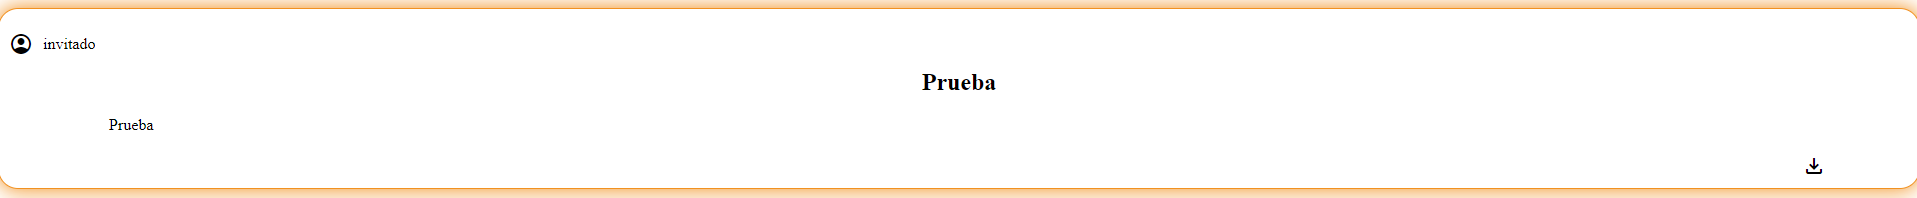
\includegraphics[width=1\textwidth]{./img/vulnerabilidades/2.1/1.1.png}
                    \caption{Evento creado mediante URL}
                \end{figure}

                Este tipo de vulnerabilidad es muy peligrosa ya que permite a un atacante crear contenido en la pagina web sin necesidad de autenticarse y de forma masiva.
                Esto puede llevar a que un atacante pueda crear contenido malicioso en la pagina web y afectar a los usuarios que visiten la pagina.               
            \clearpage
        \section{Fallos criptográficos}
            \subsection{Sniffing}
                El Sniffing es un ataque que consiste en capturar el trafico de una red para obtener informacion sensible.\\
                Dado que la pagina web no hace uso de HTTPS, podemos realizar un ataque de tipo Sniffing para obtener los datos de un usuario.
                Para ello, vamos a utilizar la herramienta Wireshark.
                Wireshark es un analizador de protocolos de red que nos permite capturar y analizar el trafico de una red.\\

                En este caso, voy a intentar iniciar sesion en la pagina web y capturar el trafico para ver si puedo obtener la contraseña.
                Dado que wireshark permite varias interfaces de captura, en mi caso, al estar corriendo el contenedor en local, voy a utilizar la interfaz de loopback.
                En un ataque real es importante hacer uso bien de la interfaz ethernet en caso de usar cable o de la interfaz wifi en caso de usar una red inalambrica.
                \begin{figure}[H]
                    \centering
                    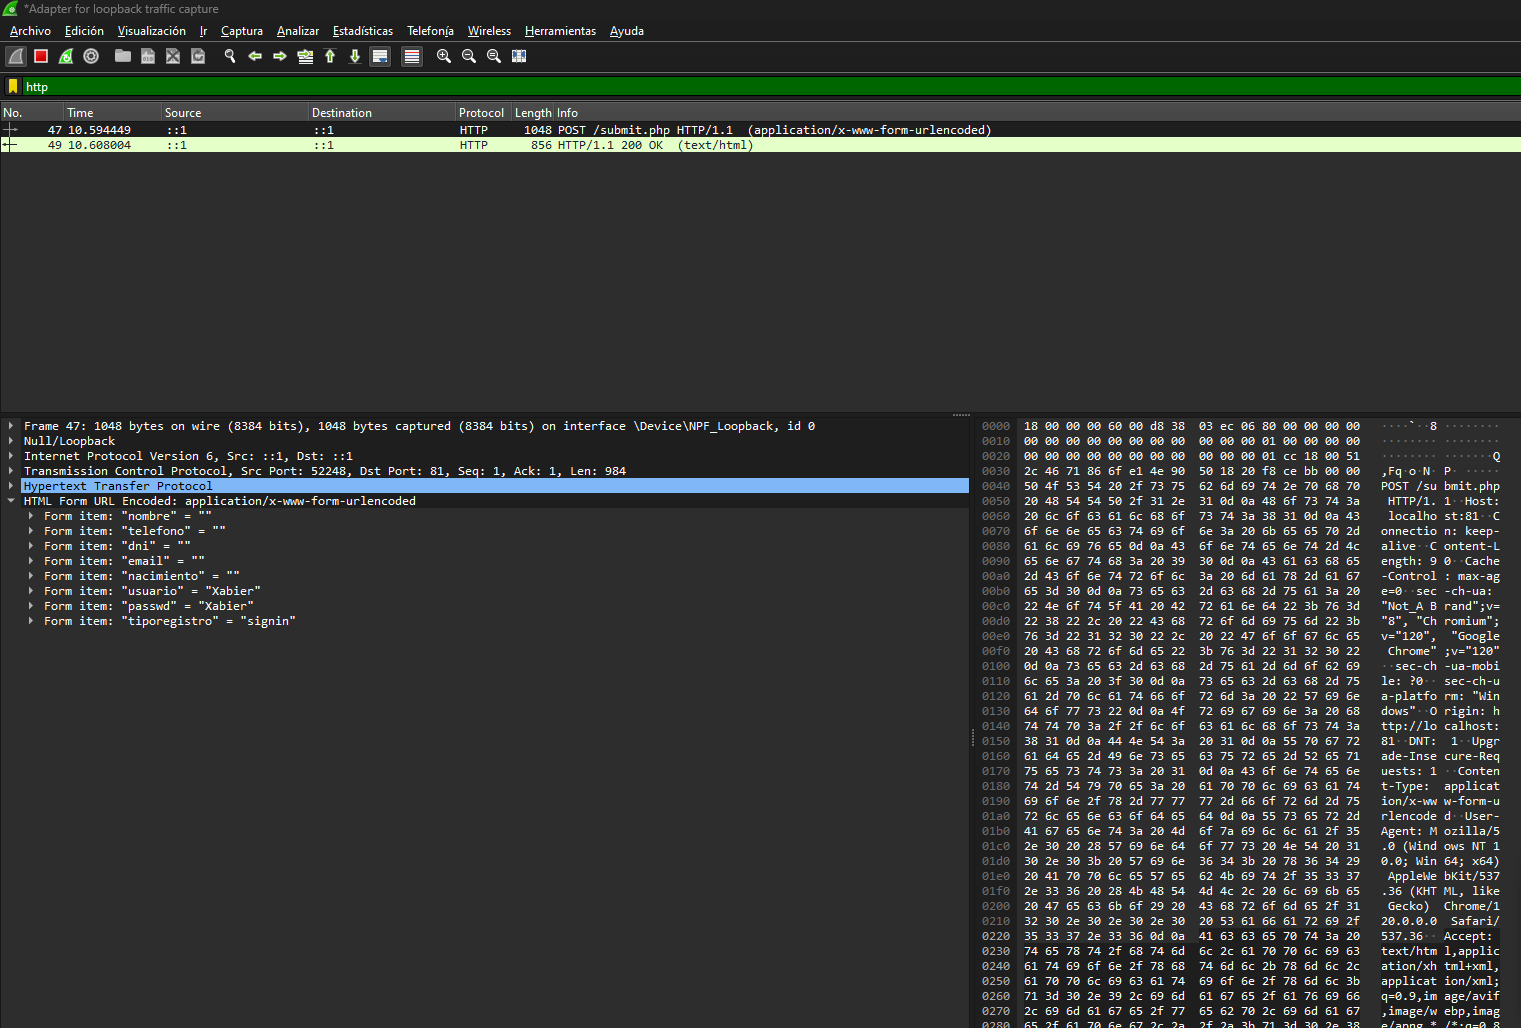
\includegraphics[width=1\textwidth]{./img/vulnerabilidades/2.2/1.1.png}
                    \caption{Captura de trafico con Wireshark}
                \end{figure}
                Como podemos ver en la imagen, en el paquete se envia el usuario y la contraseña en texto plano.
                Esto no daria acceso a un atacante a la cuenta de un usuario.\\
            \clearpage
            \subsection{MITM}
                Un ataque MITM o Man in the Middle es un ataque que consiste en interceptar el trafico de una red e inyectar o modificar paquetes.
                En este caso, vamos a realizar un ataque MITM para modificar el trafico de la red y poder modificar las publicaciones de un usuario.
                Para ello, hare uso de la herramienta Burp Suite.
                Burp Suite es una herramienta muy completa que nos permite realizar ataques MITM, analizar el trafico de una red, realizar ataques de tipo XSS, etc.\\

                Para realizar el ataque, vamos a utilizar el navegador de Burp Suite que viene preconfigurado con un proxy para poder realizar el ataque MITM.
                Primero de todo accedemos a la pagina web y vamos crear un evento.
                \begin{figure}[H]
                    \centering
                    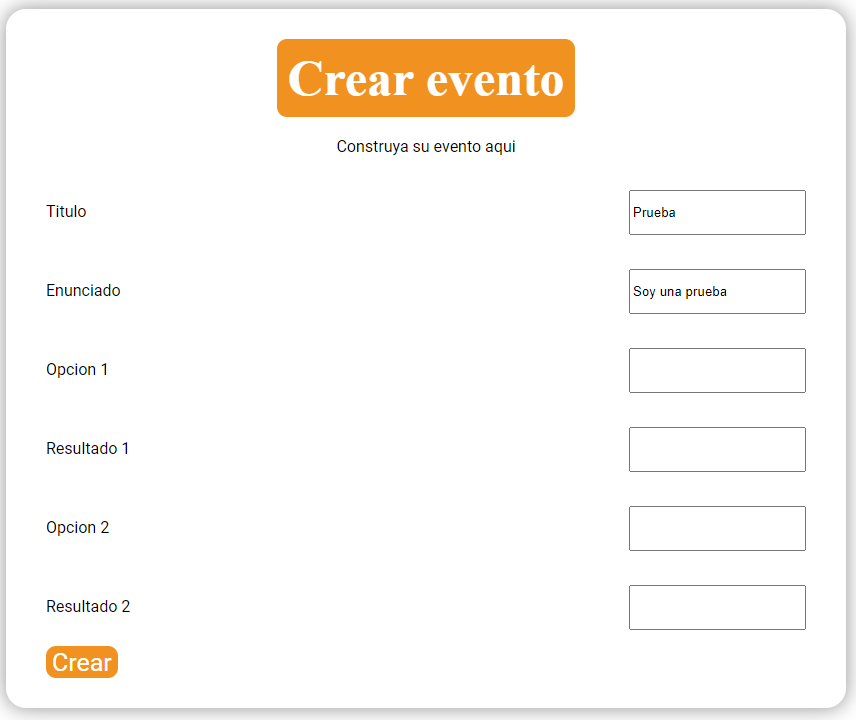
\includegraphics[width=1\textwidth]{./img/vulnerabilidades/2.2/2.1.png}
                    \caption{Creación de evento}
                \end{figure}
                \clearpage
                Antes de darle al boton de crear, vamos a decirle a Burp Suite que active el intercept para que nos muestre los paquetes que se envian.
                \begin{figure}[H]
                    \centering
                    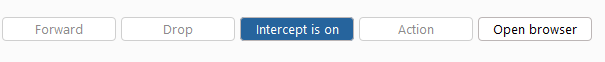
\includegraphics[width=1\textwidth]{./img/vulnerabilidades/2.2/2.2.png}
                    \caption{Activación del intercept}
                \end{figure}
                Una vez activado, le damos al boton de crear y nos aparecera el paquete que se envia.
                \begin{figure}[H]
                    \centering
                    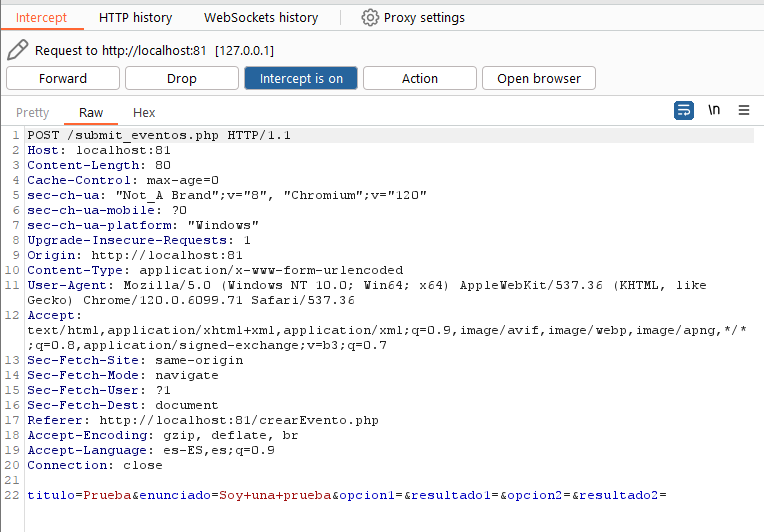
\includegraphics[width=1\textwidth]{./img/vulnerabilidades/2.2/2.3.png}
                    \caption{Paquete enviado}
                \end{figure}
                \clearpage
                Como podemos ver, el paquete contiene el titulo y la descripcion del evento en texto plano.
                Esto nos permite modificar el contenido del evento antes de que se cree.
                Para ello, vamos a modificar el titulo del evento y le damos al boton de 'Forward'.
                \begin{figure}[H]
                    \centering
                    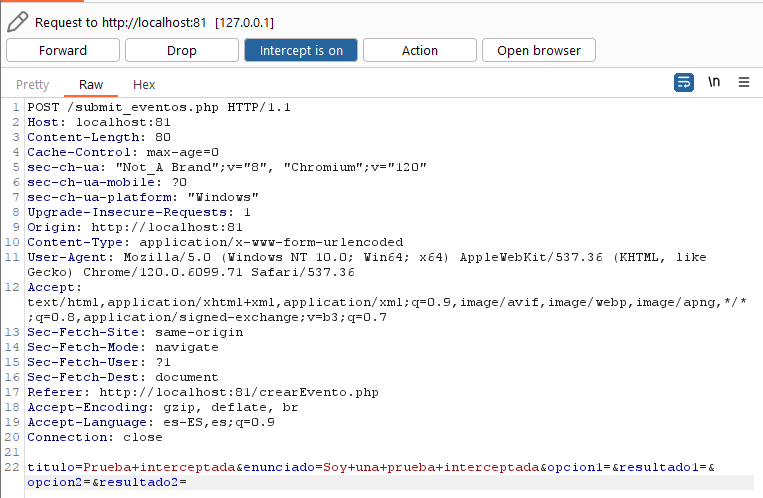
\includegraphics[width=1\textwidth]{./img/vulnerabilidades/2.2/2.4.png}
                    \caption{Modificación del paquete}
                \end{figure}
                Ahora al acceder a la pagina web, podemos ver que el titulo del evento ha cambiado por el que hemos puesto nosotros.
                \begin{figure}[H]
                    \centering
                    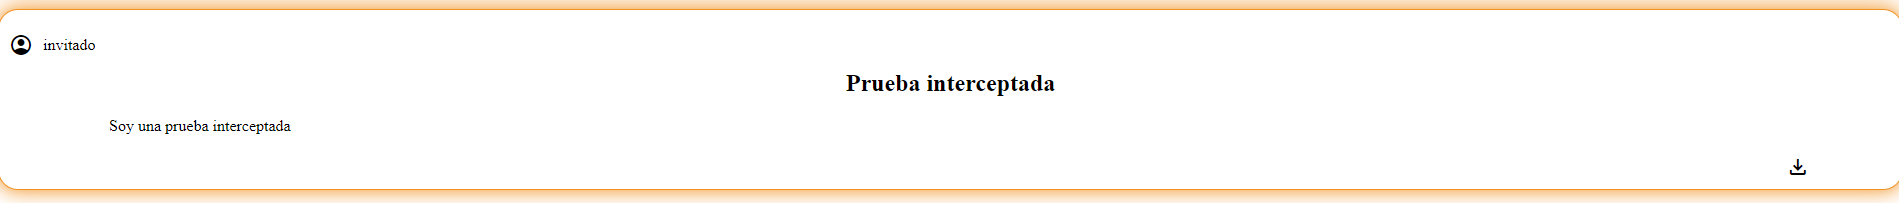
\includegraphics[width=1\textwidth]{./img/vulnerabilidades/2.2/2.5.png}
                    \caption{Evento modificado}
                \end{figure}
                Este tipo de ataque es muy peligroso ya que nos permite modificar el contenido de la pagina web y realizar acciones en nombre de la victima.
                En este caso, hemos modificado el titulo de un evento, pero podriamos haber modificado cualquier otro campo de la pagina web llegando a poder afectar al usuario.
            \clearpage
        \section{Inyecciones}
            \subsection{SQL Injection}
                La primera vulnerabilidad que vamos a probar es la de SQL Injection con la intencion de obtener información de la base de datos.
                Para el analisis de esta vulnerabilidad vamos a utilizar la herramienta sqlmap. 
                Esta herramienta nos permite analizar una url y comprobar si es vulnerable a SQL Injection de forma sencilla y automatizada.
                Una vez instalada, hemos ejecutado el siguiente comando para realizar las pruebas:\\
                \begin{center}
                    \texttt{sqlmap -u http://localhost:81/login.php --wizard}
                \end{center}
                Este analisis nos ha dado como resultado que la url es vulnerable a 3 tipos de SQL Injection:
                \begin{itemize}
                    \item Boolean-based blind SQL injection
                    \item Error-based SQL injection
                    \item Time-based blind SQL injection
                \end{itemize}
                \begin{figure}[H]
                    \centering
                    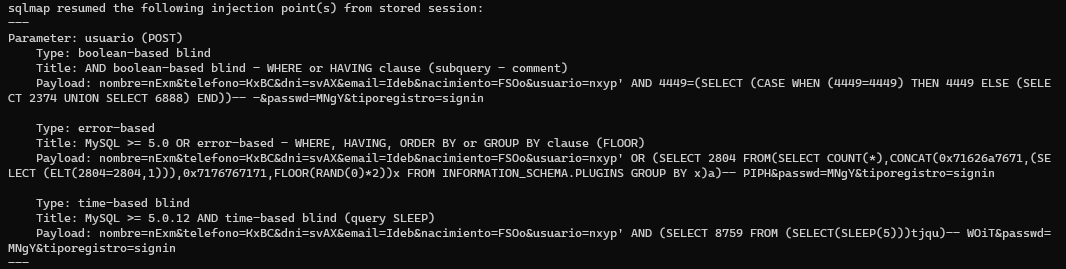
\includegraphics[width=1\textwidth]{./img/vulnerabilidades/2.3/1.1.png}
                    \caption{Puntos de injección}
                \end{figure}
                \clearpage
                Y es mediante el uso de estas vulnerabilidades que sqlmap, automaticamente, ha conseguido obtener las dos tablas de la base de datos:
                \begin{figure}[H]
                    \centering
                    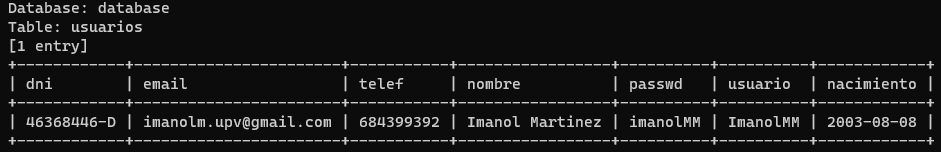
\includegraphics[width=1\textwidth]{./img/vulnerabilidades/2.3/1.2.png}
                    \caption{Tabla usuarios de la base de datos}
                \end{figure}
                \begin{figure}[H]
                    \centering
                    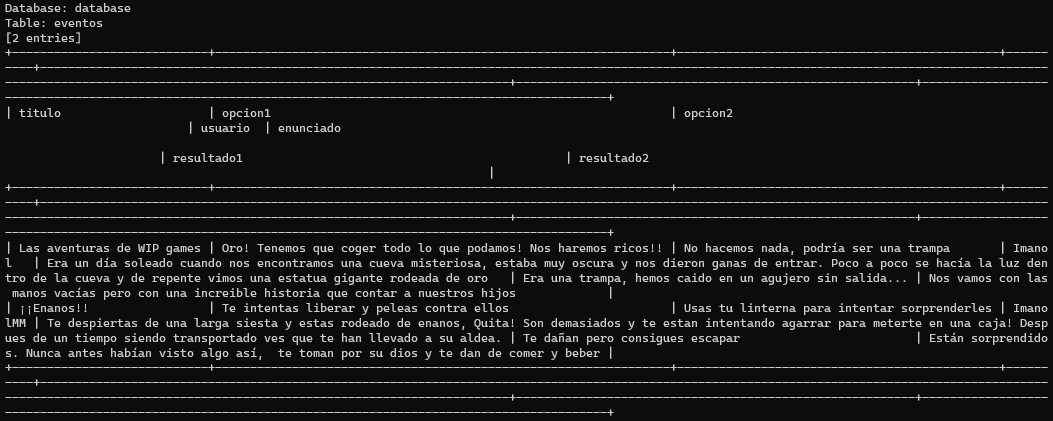
\includegraphics[width=1\textwidth]{./img/vulnerabilidades/2.3/1.3.png}
                    \caption{Tabla eventos de la base de datos}
                \end{figure}
                \clearpage
            \subsection{Cross Site Scripting}
                Tal y como hemos visto en la Introducción mediante el uso de ZAP hemos encontrado una vulnerabilidad de tipo XSS.
                En este caso, vamos a explotarlas de forma manual para ver que podemos hacer con ellas.
                Para ello accedemos al menu de 'Crear Evento' y en el campo 'Titulo' podemos introducir los siguientes codigos:
                \begin{enumerate}
                    \item \texttt{<script>alert("XSS")</script>}
                    \begin{itemize}
                        \item Este codigo nos muestra un mensaje de alerta con el texto 'XSS'
                        \begin{figure}[H]
                            \centering
                            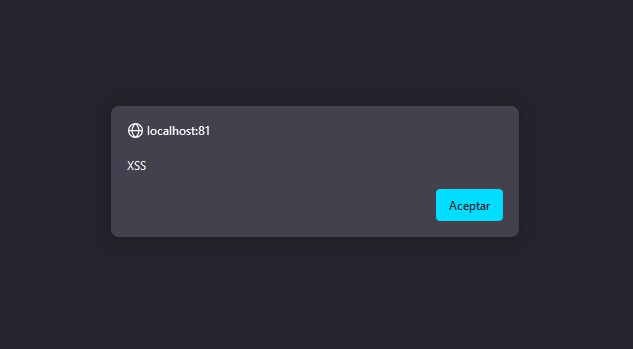
\includegraphics[width=1\textwidth]{./img/vulnerabilidades/2.3/2.1.png}
                            \caption{Alerta XSS}
                        \end{figure}
                    \end{itemize}
                    \item \texttt{<script>document.location="https://github.com/Xabierland"</script>}
                    \begin{itemize}
                        \item Este codigo nos redirige a mi pagina de Github
                    \end{itemize}
                    \item \texttt{<img src="https://shorturl.at/avFJO">}
                    \begin{itemize}
                        \item Este codigo nos muestra una imagen con el texto Pwned!
                        \begin{figure}[H]
                            \centering
                            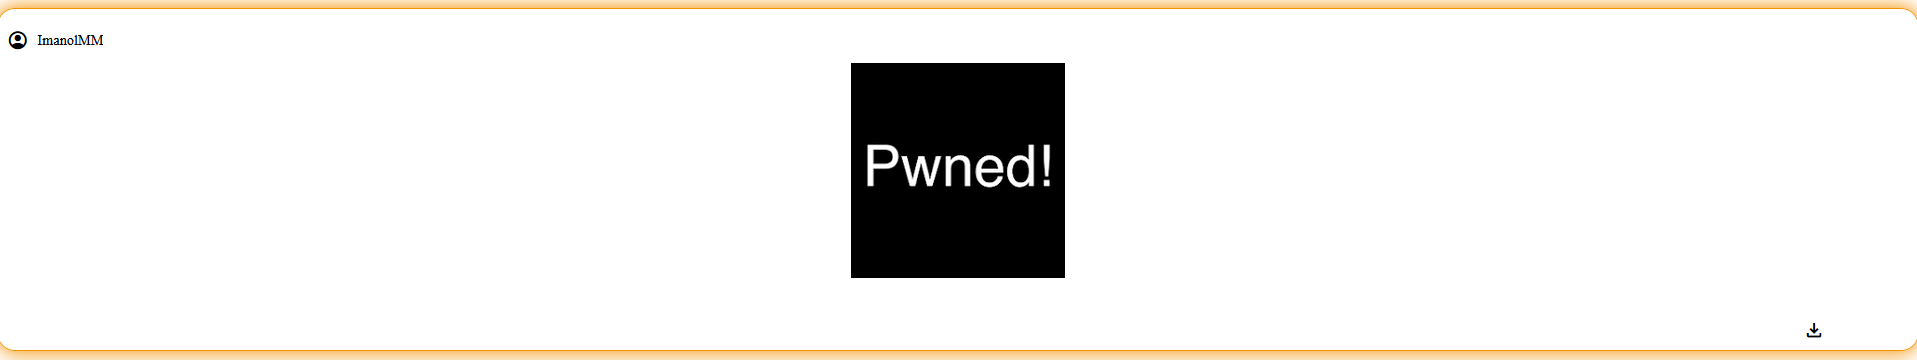
\includegraphics[width=1\textwidth]{./img/vulnerabilidades/2.3/2.3.png}
                            \caption{Imagen XSS}
                        \end{figure}
                    \end{itemize}
                    \item \texttt{<script>var paragraph = document.createElement('p');paragraph.textContent = 'Cookie: ' + document.cookie;document.body.appendChild(paragraph);</script>}
                    \begin{itemize}
                        \item Este codigo nos muestra el contenido de la cookie de php
                        \begin{figure}[H]
                            \centering
                            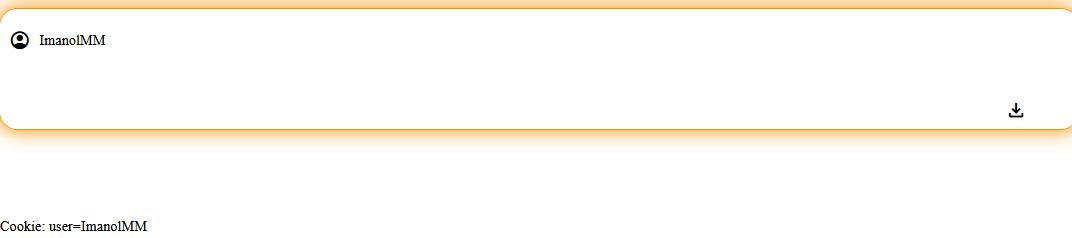
\includegraphics[width=1\textwidth]{./img/vulnerabilidades/2.3/2.4.png}
                            \caption{Cookie XSS}
                        \end{figure}
                    \end{itemize}
                \end{enumerate}
                Este tipo de vulnerabilidad es muy peligrosa ya que permite a un atacante ejecutar codigo en el navegador de la victima y realizar acciones en su nombre.\\

                Tambien hemos visto que podemos redirigir a la victima a una pagina maliciosa, lo que nos permitiria realizar un ataque de tipo Phishing.\\

                Aunque la carga de la imagen no parezca muy peligrosa, esta, en realidad puede darnos informacion como la IP de los usuarios que visitan la pagina ya que para cargar dicha imagen se realiza una peticion al servidor donde esta alojada dejando su IP en el camino.\\

                En este caso, hemos visto que podemos llegar incluso a ver la cookie de la victima, lo que nos permitiria hacer un ataque de tipo Session Hijacking.\\
                
                \clearpage
        \section{Configuración de seguridad insuficiente}
            \subsection{Fuga de información}
                La fuga de informacion es un problema muy comun en las paginas web.
                En este caso, vamos a ver como podemos obtener informacion sensible de la pagina web.\\

                Para empezar obtenedremos informacion del servidor como son el tipo de servidor y el sistema operativo.
                Para esto vamos a utilizar la herramienta Nmap.
                Nmap es un escaner de puertos que nos permite obtener informacion de los servicios que se estan ejecutando en un servidor.
                \begin{center}
                    \texttt{sudo nmap -sV -O localhost}
                \end{center}
                \begin{figure}[H]
                    \centering
                    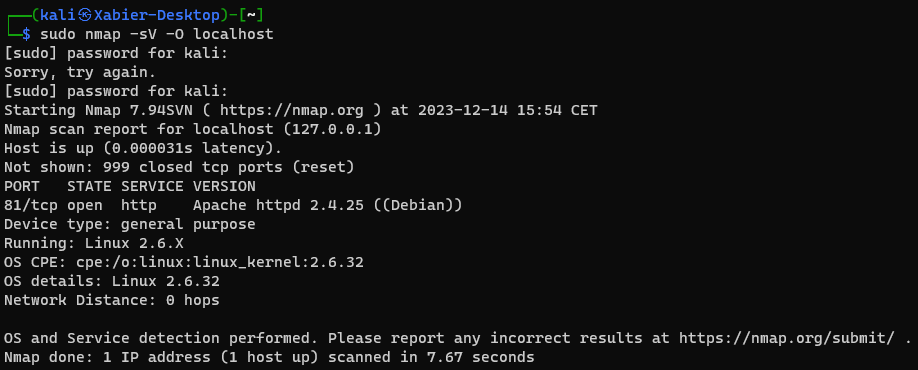
\includegraphics[width=1\textwidth]{./img/vulnerabilidades/2.4/1.1.png}
                    \caption{Información del servidor}
                \end{figure}
                Como podemos ver el servidor esta ejecutando Apache 2.4.25 en un sistema operativo Debian con una version de Kernel 2.6.32.\\
                Esta es informacion muy valiosa para un atacante ya que le permite saber que vulnerabilidades puede explotar para atacar el servidor.\\
                \clearpage
                Ahora vamos a ver si podemos obtener informacion de la version de PHP que esta ejecutando el servidor.
                Para ello, en vez de la herramienta Nmap, vamos a fijarnos en las cabeceras HTTP que nos devuelve el servidor.
                Para ello, vamos a utilizar la herramienta curl.
                \begin{center}
                    \texttt{curl -I localhost:81}
                \end{center}
                \begin{figure}[H]
                    \centering
                    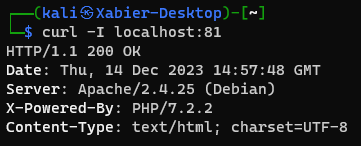
\includegraphics[width=1\textwidth]{./img/vulnerabilidades/2.4/1.2.png}
                    \caption{Cabeceras HTTP}
                \end{figure}
                Como podemos ver, en las cabeceras HTTP nos devuelve la version de PHP que esta ejecutando el servidor es la 7.2.2.
                Esta informacion al igual que la anterior, la cual se verifica en la cabecera, es muy valiosa para un atacante.\\

                El llegar a conocer toda esta informacion del servidor es una brecha importante de seguridad.

            \clearpage
            \subsection{Enumeración de directorios}
                La enumeración de directorios es un ataque que consiste en obtener informacion de los directorios que hay en el servidor.
                Para ello, vamos a utilizar la herramienta DirBuster.
                DirBuster es una herramienta que nos permite enumerar los directorios de un servidor web basado en fuerza bruta y diccionarios.
                En este caso voy a utilizar el diccionario 'directory-list-2.3-medium.txt' que viene por defecto con la herramienta.
                \begin{figure}[H]
                    \centering
                    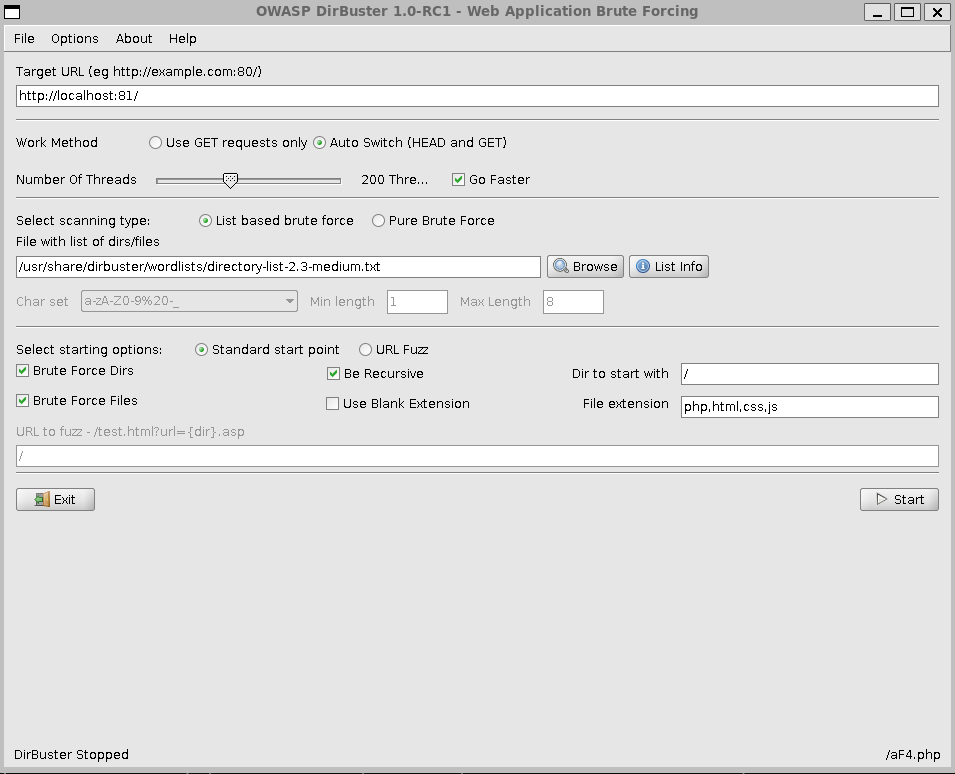
\includegraphics[width=1\textwidth]{./img/vulnerabilidades/2.4/2.1.png}
                    \caption{DirBuster}
                \end{figure}
                En la imagen se ve que ademas de dar la direccion del servidor y el diccionario he pedido que busque elemtnos de tipo php, html, css y js.
                \clearpage
                Una vez terminado el escaneo con 4.410.965 de nombres de archivos y directorios, DirBuster nos ha dado los siguientes resultados:
                \begin{figure}[H]
                    \centering
                    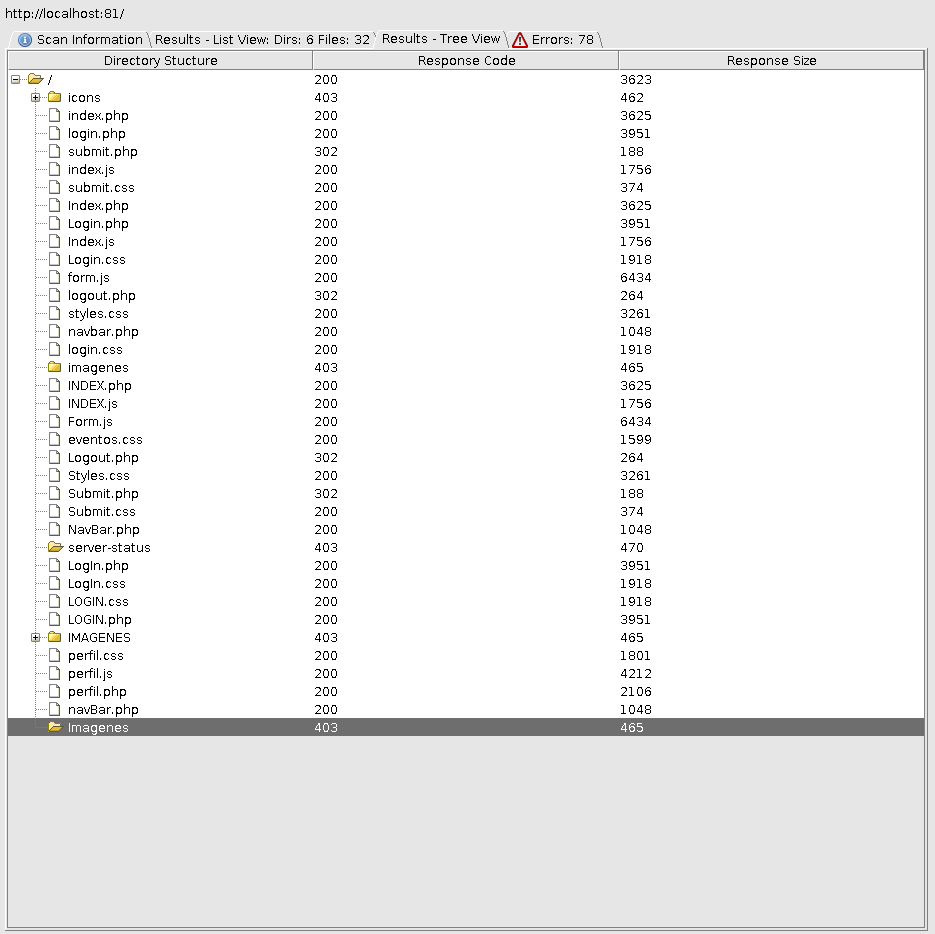
\includegraphics[width=1\textwidth]{./img/vulnerabilidades/2.4/2.2.png}
                    \caption{Resultados de DirBuster}
                \end{figure}
                Como podemos ver, DirBuster nos ha dado una lista de directorios que existen en el servidor.
                Aunque en esta lista no esten todos los directorios que existen en el servidor, si que nos da una idea de que directorios existen y cuales no.
                Esta informacion es muy valiosa para un atacante ya que le permite saber que directorios puede atacar para intentar obtener informacion sensible.\\
                

            \clearpage
            \subsection{Fuerza bruta}
            \clearpage
        \section{Componentes vulnerables y obsoletos}
            \subsection{Vulnerabilidades mediante MF}
            \clearpage
        \section{Fallos de identificación y autenticación}
            \subsection{Invalidación de sesiones}
            \clearpage
    \chapter{Bibliografia}
\end{document}